	\documentclass[20pt, a4paper]{extarticle}
	\usepackage[landscape]{geometry}
	\usepackage[portuguese]{babel}
	\usepackage[utf8]{inputenc}
	\usepackage{enumitem}
	\usepackage{capt-of}
	\usepackage{multicol}
	\usepackage{fancyhdr}
	\usepackage{lastpage}
	\usepackage{amsmath}
	\usepackage{adjustbox}
	\usepackage{amssymb}
	\usepackage{commath}
	\usepackage{graphicx}
	\usepackage{caption}
	\usepackage{float}
	\usepackage{cancel}
	\usepackage{efbox}
	\usepackage{pgfplots}
	\pgfplotsset{compat=1.18}
	\usepackage{tikz, tikz-3dplot, tkz-euclide}
	\usetikzlibrary{folding, 3d, patterns, math, calc, angles, quotes, intersections, through,datavisualization.formats.functions}
\newlist{questoes}{enumerate}{4}
\setlist[questoes]{label*=\textbf{Exercício \arabic*.}}
\begin{document}
\begin{questoes}
\item
\begin{center}\captionof{figure}{$a_{n} = \text{$\frac{1}{n}$}$}
\adjustbox{valign=t}{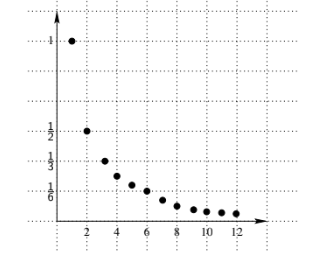
\includegraphics[width=0.5\textwidth]{images/an.png}} 
\label{fig:an}
\end{center}
\centering \textbf{A sucessão $a_{n}$ é limitada e monótona portanto convergente}

\begin{center}\captionof{figure}{$b_{n} = \text{$\frac{5n+3}{n}$}$}
	\adjustbox{valign=t}{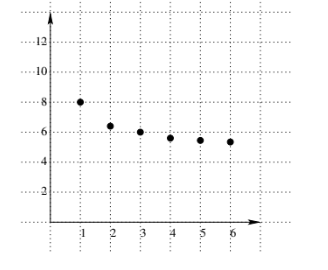
\includegraphics[width=0.5\textwidth]{images/bn.png}} 
	\label{fig:bn}
\end{center}
\centering \textbf{A sucessão $b_{n}$ é limitada e monótona portanto convergente}

\begin{center}\captionof{figure}{$c_{n} = \text{$\frac{3\left(-1\right)^n+2n}{n}$}$}
	\adjustbox{valign=t}{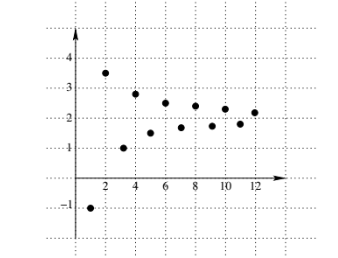
\includegraphics[width=0.5\textwidth]{images/cn.png}} 
	\label{fig:cn}
\end{center}
\centering \textbf{A sucessão $c_{n}$ é limitada, não monótona mas convergente}

\begin{center}\captionof{figure}{$d_{n} = \begin{cases}
			\text{n + 2,  se n $<$ 5}\\ 
			\text{5 se, n $\geq$ 5 }    
		\end{cases}$}
	\adjustbox{valign=t}{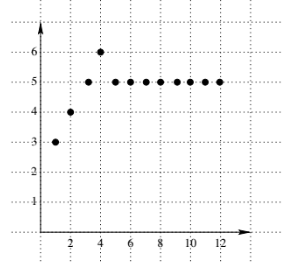
\includegraphics[width=0.5\textwidth]{images/dn.png}} 
	\label{fig:dn}
\end{center}
\centering \textbf{A sucessão $d_{n}$ é limitada, não monótona mas convergente}

\begin{center}\captionof{figure}{$e_{n} = \text{$-2^n$}$}
	\adjustbox{valign=t}{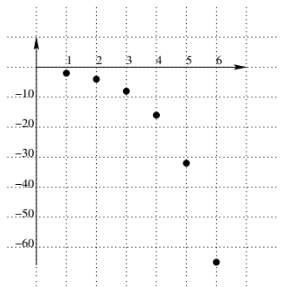
\includegraphics[width=0.5\textwidth]{images/en.png}} 
	\label{fig:en}
\end{center}
\centering \textbf{A sucessão $e_{n}$ não é limitada, é monótona e não convergente}

\begin{center}\captionof{figure}{$f_{n} = \text{$\frac{-3}{2^n}$}$}
	\adjustbox{valign=t}{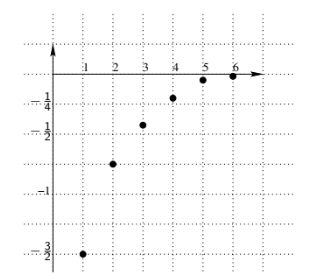
\includegraphics[width=0.5\textwidth]{images/fn.png}} 
	\label{fig:cn}
\end{center}
\centering \textbf{A sucessão $f_{n}$ é limitada e monótona portanto convergente}
\bigskip
\item \text{Considere a sucessão de termo geral $a_{n}= 3-2n$}
\begin{enumerate}[label=\alph*)]
\item \text{Determine os três primeiros termos da sucessão.}
\[a_{1}= 3-2\cdot{1}=1\]
\[a_{2}= 3-2\cdot{2}=-1\]
\[a_{3}= 3-2\cdot{3}=-3\]
\item \text{Averigue se -17 é termo da sucessão.}
\[3-2n=-17\]
\[n = 10 \]
\text{Confirmação:}
\[a_{10}= 3-2\cdot{10}=-17\]
\item \text{Estude a sucessão $a_{n}$ quanto à monotonia.}
\[a_{n+1}-a_{n}\]
\[= 3-2\left(n+1\right)-\left(3-2n\right)\]
\[= 3-2n-2-3+2n\]
\[= -2<0\]
\text{$a_{n}$ é uma sucessão monótona decrescente}

\item \text{A sucessão é limitada ?}
\[\lim\limits_{n} \left(3-2n\right)=-\infty\]
\text{$u_{n}$ É uma sucessão majorada}
\[u_{1}=1\]
\text{Seja M $\in \mathbb{R^-}$}

\[a_{n} < M\]
\[\Leftrightarrow 3-2n < M\]
\[\Leftrightarrow n > \frac{3-M}{2}\]	

\begin{tikzpicture}[scale=1.5][master]
	\begin{axis}[
		enlargelimits=0.2,
		]
		\addplot+ [nodes near coords,only marks,
		point meta=explicit symbolic]
		table [meta=label] {
			x    y   label
			1     1   $a_{1}$
			2    -1   $a_{2}$
			3    -3   $a_{3}$
			4    -5   $a_{4}$
			5    -7   $a_{5}$
			6    -9   $a_{6}$
			7    -11  $a_{7}$
			8    -13  $a_{8}$
			9    -15  $a_{9}$
		};
	\end{axis}
	\end{tikzpicture}
\end{enumerate}
\item \text{Considere a sucessão de termo geral $u_{n}= \frac{3n-2}{n}$}
\begin{enumerate}[label=\alph*)]
	\item \text{Determine os dois primeiros termos da sucessão.}
	\[u_{1}= \frac{3\left(1\right)-2}{1}=1\]
	\[u_{2}= \frac{3\left(2\right)-2}{2}=2\]
	\item \text{Verifique se $\frac{5}{2}$ é termo da sucessão.}
	\[3-\frac{2}{n}=\frac{5}{2}\]
	\[n = 4\]
	\text{Como n $\in \mathbb{N}$, então é termo da sucessão}
	\item \text{Estude a sucessão $u_{n}$ quanto à monotonia.}
	\[u_{n+1}-u_{n}\]
	\[= \frac{3\left(n+1\right)-2}{n+1}-\left(\frac{3n-2}{n}\right)\]
	\[= \left[\frac{3n+1}{n+1}\right]\cdot \left[\frac{n}{n}\right]-\left[\frac{3n-2}{n}\right]\cdot \left[\frac{n+1}{n+1}\right]\]
	\[= \frac{2}{\left(n+1\right)\left(n\right)}>0\]
	\text{$u_{n}$ é uma sucessão crescente}
	\item \text{A sucessão é limitada ?}
	\[3-\frac{2}{n}\]
	\[-\frac{2}{n}<0\]
	\[1<3-\frac{2}{n}<3\]
	\text{$u_{n}$ é uma sucessão monótona, limitada}

\begin{tikzpicture}[scale=1.5][master]
		\begin{axis}[
			enlargelimits=0.2,
			]
			\addplot+ [nodes near coords,only marks,
			point meta=explicit symbolic]
			table [meta=label] {
				x    y   label
				1     1  $u_{1}$
				2     2  $u_{2}$
				3     2.3333  $u_{3}$
				4     2.5  $u_{4}$
				5     2.6 $u_{5}$
				6     2.6666 $u_{6}$
				7     2.71428 $u_{7}$
				8     2.75 $u_{8}$
				9     2.7777777777777777 $u_{9}$
			};
		\end{axis}
	\end{tikzpicture}
\end{enumerate}

\item \text{Considere a sucessão de termo geral $b_{n}= n^2-8n$}
\begin{enumerate}[label=\alph*)]
	\item \text{Determine os quatro primeiros termos da sucessão.}
	\[b_{1}= \left(1\right)^2-8=-7\]
	\[b_{2}= \left(2\right)^2-16=-12\]
	\[b_{3}= \left(3\right)^2-24=-15\]
	\[b_{4}= \left(4\right)^2-32=-16\]
	\item \text{Calcule o vigésimo termo da sucessão e diga se a sucessão é monótona.}
	\[b_{20}= \left(20\right)^2-160=240\]
	
	\text{$b_{n}$  não é uma sucessão monótona}
\end{enumerate}
\item
\begin{enumerate}[label=\alph*)]
	\item \[\lim\limits_{n}\ \left(\frac{2+3n}{5n}\right) \overset{\mathrm{\frac{0}{0}}}{=} \lim\limits_{n}\ \left(\frac{\cancel{n}\left(\cancelto{0}{\frac{2}{n}}+3\right)}{\cancel{n}\left(5\right)}\right) = \frac{3}{5}\]
	
	\item \[\lim\limits_{n}\ \left(\frac{3n^2+4n-2}{4n^2-3n+5}\right) \overset{\mathrm{\frac{\infty}{\infty}}}{=}
	\lim\limits_{n} \left(\frac{\cancel{n^2}\left(3+\cancelto{0}{\frac{4}{n}}-\cancelto{0}{\frac{2}{n^2}}\right)}{\cancel{n^2}\left(4-\cancelto{0}{\frac{3}{n}}+\cancelto{0}{\frac{5}{n^2}}\right)}\right) =\frac{3}{4}\]
	
	\item \[\lim\limits_{n}\ \left(\frac{3n^2+1}{4n^3+5}\right) \overset{\mathrm{\frac{\infty}{\infty}}}{=}	\lim\limits_{n}\ \left(\frac{\cancel{n^2}\left(3+\cancelto{0}{\frac{1}{n^2}}\right)}{n\cancel{^3}\left(4+\cancelto{0}{\frac{5}{n^3}}\right)}\right) \]
	\[\lim\limits_{n}\ \left(\frac{3}{4n}\right) = \frac{3}{+\infty} = 0\]
	
	\item \[\lim\limits_{n}\ \left(\frac{3n^3+4n^2-3n+2}{4n^2+3n+2}\right) \overset{\mathrm{\frac{\infty}{\infty}}}{=} \lim\limits_{n}\ \left(\frac{n\cancel{^3}\left(3+\cancelto{0}{\frac{4}{n}}-\cancelto{0}{\frac{3}{n^2}}+\cancelto{0}{\frac{2}{n^3}}\right)}{\cancel{n^2}\left(4+\cancelto{0}{\frac{3}{n}}+\cancelto{0}{\frac{2}{n^2}}\right)}\right)\]
	\[ = \lim\limits_{n}\ \left(\frac{3n}{4}\right) = \frac{+\infty}{4} +\infty\]
	
	\item \[\lim\limits_{n}\ \left(5\left(-1\right)^n\right) \begin{cases}
		\text{-5 se n é ímpar}\\ 
		\text{5 se n é par}    
	\end{cases}
\text{Limite não existe}
\]
	\item \[\lim\limits_{n}\ \left(\sqrt{n^3+3}\right) = \sqrt{\left(\infty\right)^3+3} = +\infty\]
	
	\item \[\lim\limits_{n}\ \frac{\sqrt{4n^2+1}}{n+3} \overset{\mathrm{\frac{\infty}{\infty}}}{=} \lim\limits_{n}\	 \frac{\sqrt{n^2\left(4+\frac{1}{n^2}\right)}}{n\left(1+\frac{3}{n}\right)} =\lim\limits_{n}\ \frac{\cancel{n}\sqrt{4+\cancelto{0}{\frac{1}{n^2}}}}{\cancel{n}\left(\cancelto{0}{1+\frac{3}{n}}\right)}= 2\]
	
	\item \[\lim\limits_{n}\ \left(\frac{1}{\sqrt{n^2+1}}-\frac{1}{\sqrt{n^2+2}}\right)\]
	\[\frac{1}{\sqrt{+\infty}} - \frac{1}{\sqrt{+\infty}}\]
	\[= 0 - 0 = 0\]
	
	\item \[\lim\limits_{n}\ \left(\frac{1}{\sqrt{n^4+2}-\sqrt{n^4+3}}\right) \overset{\mathrm{\infty-\infty}}{=}\]\[\lim\limits_{n}\  \left(\frac{\sqrt{n^4+2}+\sqrt{n^4+3}}{\left(\sqrt{n^4+2}-\sqrt{n^4+3}\right)\left(\sqrt{n^4+2}+\sqrt{n^4+3}\right)}\right)\] 
	\[=\lim\limits_{n}\ \left(\frac{\sqrt{n^4+2}+\sqrt{n^4+3}}{-1}\right)\] 
	\[=-\lim\limits_{n}\ \left(\sqrt{n^4+2}+\sqrt{n^4+3}\right)\]
	\[=-\left(\sqrt{+\infty}+\sqrt{+\infty}\right) = - \infty\]
	\item \[\lim\limits_{n}\ \left(\sqrt{n^2+2}-\sqrt{n^2-n}\right)\overset{\mathrm{\infty-\infty}}{=}\]
	
	\[=\lim\limits_{n}\ \left(\frac{\left(\sqrt{n^2+2}-\sqrt{n^2-n}\right)\left(\sqrt{n^2+2}+\sqrt{n^2-n}\right)}{\left(\sqrt{n^2+2}+\sqrt{n^2-n}\right)}\right)\]
	
	\[=\lim\limits_{n}\ \left(\frac{2+n}{\left(\sqrt{n^2+2}+\sqrt{n^2-n}\right)}\right)\]
	
	\[=\lim\limits_{n}\ \left(\frac{n\left(\frac{2}{n}+1\right)}{\sqrt{n^2\left(1+\frac{2} {n^2}\right)}+{\sqrt{n^2\left(1-\frac{1} {n}\right)}}}\right)\]
	
	\[=\lim\limits_{n}\ \left(\frac{\cancel{n}\left(\cancelto{0}{\frac{2}{n}}+1\right)}{\cancel{n}\left(\sqrt{1+\cancelto{0}{\frac{2}{n^2}}}+{\sqrt{1-\cancelto{0}{\frac{1} {n}}}}\right)}\right)\]
	\[=\frac{1}{2}\]
\end{enumerate}
\end{questoes}
\end{document}